\section{Тема 4} % TODO:

\subsection{Релации}

\begin{definition}
	Нека \(n \ge 1\) и \mexpr{A_1, A_2, ..., A_n} са множество, наречени съответно първи домейн,
	втори домейн, ..., \(n\)-ти домейн. \textbf{Релация} над декартовото произведение
	\mexpr{A_1 \times A_2 \times ... \times A_n} е всяко множество \mexpr{R \subseteq A_1 \times A_2 \times ... \times A_n}.
	Казваме, че \(R\) е \(n\)-местна или \(n\)-арна.
\end{definition}

\begin{example}
	\(<, \le, >, \ge, =\) са релации над декартовия квадрат \(\mathbb{R}^2\).

	Нека \(S\) е множество, \mexpr{\subseteq_{S}} е релация над \mexpr{2^S \times 2^S}, дефенирана така:
	\begin{center}
		\mexpr{\forall a, b \in 2^S: (a, b) \in \subseteq_{S} \iff a \subseteq b}
	\end{center}

	Нека \mexpr{S = \{a, b\}}. Тогава \mexpr{(\{a\}, \{a, b\}) \in \subseteq_{S}, (\{a, b\}, \{a\}) \not \in \subseteq_{S}} и т.н.
\end{example}

\subsection{Двуместни релации над декартови квадрати и представяне чрез матрици и графи (диаграми)}

Нека \mexpr{A = \{a_1, a_2, ..., a_n\}} и \mexpr{R \subseteq A^2}.
Например, \mexpr{A = \{a, b, c, d\}, R = \{(a, a), (a, b), (c, c), (d, a)\}}.

\begin{scheme}[Представяне чрез матрици]
	Можем да представим \(R\) чрез булева матрица \(n \times n\), в която на ред \(i\) и колона \(j\) е:
	\begin{itemize}
		\item 1, ако \mexpr{a_iRa_j}
		\item 0, в противен случай
	\end{itemize}

	\begin{center}
		\begin{tabular}{ | c | c | c | c | c | }
			\hline
			  & a                  & b                  & c                  & d \\
			\hline
			a & \textcolor{red}{1} & \textcolor{red}{1} & 0                  & 0 \\
			\hline
			b & 0                  & 0                  & 0                  & 0 \\
			\hline
			c & 0                  & 0                  & \textcolor{red}{1} & 0 \\
			\hline
			d & \textcolor{red}{1} & 0                  & 0                  & 0 \\
			\hline
		\end{tabular}
	\end{center}
\end{scheme}

\begin{scheme}[Представяне чрез графи]
	Можем да представим \(R\) чрез диаграма от точки и стрелки, в която на всяко \(a_i\) съответства отделна
	точка, наречена връх, а ребро от връх \(a_i\) до върха \(a_j\) има \totw \(a_iRa_j\).

	\begin{center}
		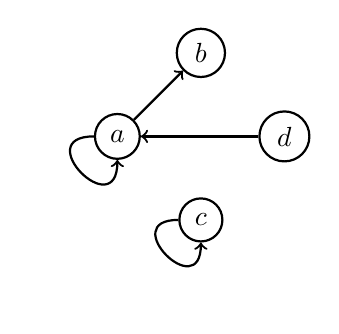
\begin{tikzpicture}[node distance={15mm}, thick, main/.style = {draw, circle}]
			\node[main] (1) {$a$};
			\node[main] (2) [above right of=1] {$b$};
			\node[main] (3) [below right of=1] {$c$};
			\node[main] (4) [above right of=3] {$d$};
			\draw[->] (1) to [out=180,in=270,looseness=5] (1);
			\draw[->] (1) -- (2);
			\draw[->] (3) to [out=180,in=270,looseness=5] (3);
			\draw[->] (4) -- (1);
		\end{tikzpicture}
	\end{center}
\end{scheme}

\subsection{Свойства на двуместни релации}
Нека \mexpr{R \subseteq A^2}.

% TODO: add matrix and graph info?
\begin{enumerate}
	\item Рефлексивност \\
	      \(R\) е рефлексивна \totw \mexpr{\forall a \in A: aRa}.

	\item Антирефлексивност \\
	      \(R\) е антирефлексивна \totw \mexpr{\forall a \in A: \lnot aRa}.

	\item Симетричност \\
	      \(R\) е симетрична \totw \mexpr{\forall a, b \in A, a \not = b: aRb \to bRa}.

	\item Антисиметричност \\
	      \(R\) е антисиметрична \totw \mexpr{\forall a, b \in A, a \not = b: aRb \to \lnot bRa}.

	\item Силна антисиметричност \\
	      \(R\) е силно антисиметрична \totw \mexpr{\forall a, b \in A, a \not = b: aRb \oplus bRa}.

	\item Транзитивност \\
	      \(R\) е транзитивна \totw \mexpr{\forall a, b \in A : aRb \land bRc \to aRc}.

\end{enumerate}

\subsection{Затваряния на релации}

\begin{definition}
	\textbf{Рефлексивното/симетричното/транзитивното затваряне} на \(R\) е минималното множество \mexpr{R^{'} \subseteq A^2},
	такова че \mexpr{R \subseteq R^{'}} и \(R^{'}\) е рефлексивна/симетрична/транзитивна релация.

	"\(R^{'}\) е минималното множество" означава, че за всяко \mexpr{R^{''} \subseteq A^2}, такова че
	\mexpr{R \subseteq R^{''}} и \(R^{''}\) е рефлексивна/симетрична/транзитивна, е вярно, че \mexpr{R^{'} \subseteq R^{''}}.

	Релация е рефлексивна/симетрична/транзитивна \totw съвпада с рефлексивното/симетричното/транзитивното си
	затваряне.
\end{definition}

\begin{additional}
	Нека \(A\) е крайно и релациите над \(A\) са представени с матрици.

	Рефлексивното затваряне се получава с едно сканиране на главния диагонал и обръщане на всяка \(0\) в \(1\).

	Симетричното затваряне се получава чрез сканиране за двойки \((0; 1)\) и \((1; 0)\), които са симетрично
	спрямо главния диагонал, и обръщане на \(0\)-та от двойката в \(1\)-ца.

	Транзитивното затваряне се получава по-сложно - нещо като умножение на матрицата със себе си \(n - 1\) пъти.
\end{additional}

\subsection{Релации на еквивалентност}

\begin{definition}
	Релация е релация на еквивалентност \totw е рефлексивна, симетрична и транзитивна.
\end{definition}

\begin{example}
	\(=\) е релация на еквивалентност над реалните числа.
\end{example}

\begin{note}
	Нека \mexpr{R \subseteq A^2} е релация на еквивалентност. За всеки елемент \mexpr{a \in A} дефенираме
	множеството \mexpr{[a] = \{b \in A | aRb\}}.
\end{note}

\subsection{Теорема за класовете на еквивалентност}

\begin{definition}
	Фамилията \mexpr{\{[a] | a \in A\}} е разбиване на \(A\). Елементите на тази фамилия се наричат
	\textbf{класове на еквивалентност}.
\end{definition}

\begin{proof}
	$ $\newline
	\begin{itemize}
		\item Всеки елемент на \(A\) е в поне един елемент на фамилията, понеже в \mexpr{\{[a] | a \in A\}}
		      \(a\) взема последователно стойностите на всички елементи от \(A\).
		\item Всеки елемент на фамилията е непразен, понеже \(R\) е рефлексивна.
		\item Всеки два различни елемента на фамилията имат празно сечение (което ще докажем).
		      \begin{lemma}
			      \mexpr{[a] \not = [b] \to [a] \cap [b] = \emptyset}
			      \begin{proof}
				      $ $\newline
				      Контрапозитивното е \mexpr{[a] \cap [b] \not = \emptyset \to [a] = [b]}. \\
				      Да допуснем, че \mexpr{[a] \cap [b] \not = \emptyset} за някои \mexpr{a, b \in A}. \\
				      Щом \mexpr{[a] \cap [b] \not = \emptyset}, то \mexpr{\exists c \in A: c \in [a] \cap [b]}. \\
				      Да разгледаме елемент \mexpr{d \in [a]}. Визуално: \\ % TODO: graphic
				      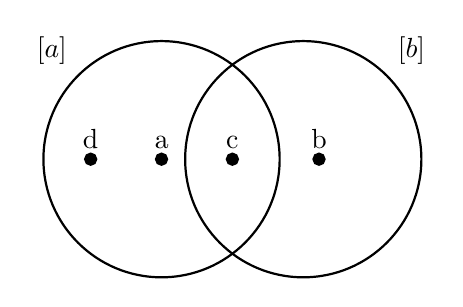
\begin{tikzpicture}[thick,
						      set/.style = {circle,
								      minimum size = 3cm,
								      fill=white}]

					      % Set [a]
					      \node[set, label={135:$[a]$}] ([a]) at (0,0) {};

					      % Set [b]
					      \node[set, label={45:$[b]$}] ([b]) at (1.8,0) {};

					      % Intersection
					      \begin{scope}
						      \clip (0,0) circle(1.5cm);
						      \clip (1.8,0) circle(1.5cm);
					      \end{scope}

					      % Circles outline
					      \draw (0,0) circle(1.5cm);
					      \draw (1.8,0) circle(1.5cm);

					      % Set points
					      \filldraw[black] (0,0) circle (2pt) node[anchor=south]{a};
					      \filldraw[black] (2,0) circle (2pt) node[anchor=south]{b};
					      \filldraw[black] (0.9,0) circle (2pt) node[anchor=south]{c};
					      \filldraw[black] (-0.9,0) circle (2pt) node[anchor=south]{d};

				      \end{tikzpicture}

				      Знаем, че \mexpr{a \in [a]} и \mexpr{b \in [b]}. \\
				      От допускането имаме, че \mexpr{(1)(c \in [a] \implies aRc)} и \mexpr{(2)(c \in [b] \implies bRc)}. \\
				      По дефиниция \mexpr{[a] = \{x \in A | aRx\}}. \\
				      Тогава: \\
				      \mexpr{aRd \implies dRa} (симетричност) \\
				      \mexpr{dRa \land aRc \to dRc} (транзитивност) \\
				      \mexpr{cRb} (симетричност и (2)) \\
				      \mexpr{dRc \land cRb \to dRb} (транзитивност) \\
				      \mexpr{dRb \implies bRd} (симетричност) \\
				      \mexpr{bRd \implies d \in [b]} \\
				      Доказахме, че \mexpr{d \in [a] \to d \in [b]} за произволен елемент \(d\). \\
				      Следователно \mexpr{[a] \subseteq [b]}. \\
				      Аналогично доказваме, че \mexpr{[b] \subseteq [a]} и от аксиомата за обема получаваме, че
				      \mexpr{[a] = [b]}.
			      \end{proof}
		      \end{lemma}
	\end{itemize}
\end{proof}